\section{SimpleITK}

\centeredlargetext{white}{black}{
SimpleITK
}


{
\setbeamertemplate{background}{}
\begin{frame}
\frametitle{SimpleITK}
\Huge
\begin{itemize}
\item Hides templates
\pause
\item Smarter IO
\pause
\item Both procedural and object-oriented interfaces
\pause
\item Easier wrapping
\pause
\item Binary distribution (\texttt{easy\_install SimpleITK})
\end{itemize}
\end{frame}
}


\begin{frame}[fragile]
  \frametitle{How to run the example?}
  \fontsize{12pt}{12pt}\selectfont
\begin{verbatim}
cd ~/src/SimpleITK-Notebooks
\end{verbatim}

\begin{verbatim}
ipython notebook --pylab=inline
\end{verbatim}
\end{frame}


\begin{frame}
  \frametitle{IPython Notebook Quickstart}
  \begin{itemize}
    \item \texttt{Shift-Enter} to run a cell
    \item \texttt{Ctrl-m h} to show keyboard shortcuts
  \end{itemize}
  \begin{center}
    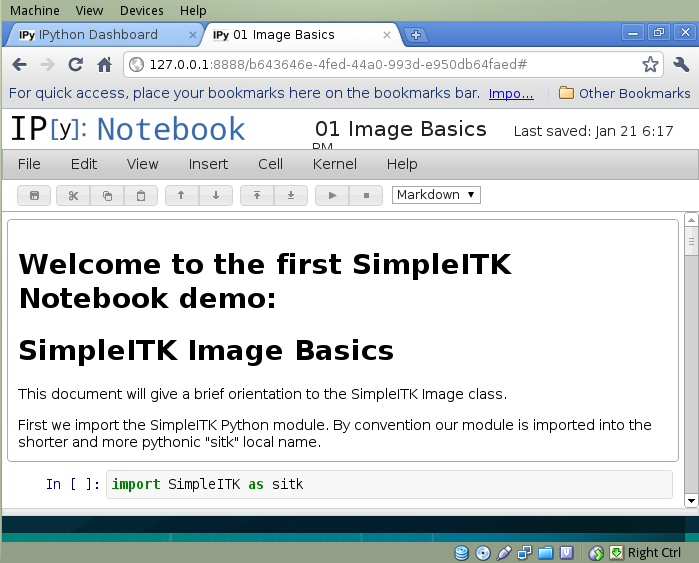
\includegraphics[width=0.5\paperwidth]{../Art/IPython-Notebook.png}
  \end{center}
\end{frame}

{
\setbeamertemplate{background}{}
\begin{frame}
\frametitle{More information on SimpleITK}
\Huge
\begin{itemize}
  \item \url{http://simpleitk.org/}
  \item \url{http://www.itk.org/Wiki/ITK_Release_4/SimpleITK}
\end{itemize}
\end{frame}
}
